% SHEAF Gate 0 white paper — substitution off, strategy off.
% Overleaf: zip this folder (main.tex, refs.bib, sections/, tables/, figures/)
% and upload (New Project → Upload Project). Compile with pdfLaTeX + BibTeX.
\documentclass[11pt,a4paper]{article}
\usepackage[margin=1in]{geometry}
\usepackage{graphicx}
\usepackage{booktabs}
\usepackage{tabularx}
\usepackage{amsmath,amssymb}
\usepackage[round,authoryear]{natbib}
\usepackage{hyperref}
\usepackage{caption}
\usepackage{subcaption}
\usepackage{float}
\usepackage{xcolor}
\usepackage{setspace}
\setstretch{1.08}

\hypersetup{colorlinks=true,linkcolor=black,citecolor=blue,urlcolor=blue}
\graphicspath{{figures/}}
\bibliographystyle{apalike}

\title{SHEAF Gate~0: a single-commodity grain-market spine\\
without substitution or strategic export restrictions}
\author{Working paper (not a journal submission)}
\date{\today}

\begin{document}
\maketitle

\begin{abstract}
SHEAF (Substitution, Heterogeneous agents, Equilibrium, And Fragility) is
designed as a multi-commodity, game-theoretic successor to TWIST and
Agrimate. Those differentiators are not exercised here. This note documents
and scores the Gate~0 spine: one crop at a time, 24 steps per year,
exogenous AMIS quantity cuts, no cross-grain substitution, no endogenous
restriction game. The mathematics, the classification of every parameter
(structural / literature / reduced-form), and the mapping to code are stated
in full. Official identification follows Agrimate's split---climatology
harvest versus LOWESS production anomalies versus anomalies plus historical
restrictions---with mean flex demand and, for maize, a USDA FSI residual for
the US Renewable Fuel Standard. World prices are compared to MUV-deflated
Pink Sheet series (constant 2010 dollars), not Agrimate's CPI-deflated
levels. On 2006--11 the matched run correlates $+0.72$ (wheat), $+0.71$
(maize), $+0.68$ (rice) with monthly Pink Sheet; 2007/08 wheat and rice
hikes are restriction-led, maize 2007/08 is industrial-demand-led, and
2010/11 wheat is production-led after detrend. A 2021--23 Ukraine-war
hindcast with locked parameters and 2019--21 FAOSTAT network structure
reproduces the wheat hike ($\times 1.61$ versus observed $\times 1.57$),
almost entirely from AMIS (India's May 2022 prohibition and Russia's
March 2022 measures), while maize and rice barely moved in the data and
the model does not invent a spike. World marketing-year-end stocks match
PSD to $\times 1.02$--$1.08$; consumption levels and some exporter shipment
\emph{volumes} versus PSD do not. The leftover list is structural. Cross-grain
substitution remains the next paper, not a repair for these residuals.
\end{abstract}

\tableofcontents
\vspace{1em}

\section{Purpose and scope}
\label{sec:scope}

SHEAF's destination is a country-level, multi-commodity network in which
governments choose export restrictions and consumers substitute across
wheat, rice, and maize~\citep{kuhla2025,schewe2017}. Collaborator feedback
and the project's own paper stack put a logically prior claim first:
before substitution or a game can be interpreted, each crop's sub-annual
market must clear, stocks must be scored at the right month, and historical
restrictions must cut offers on the nodes that actually restricted.

This note is that prior claim (Gate~0 / paper P1). It does three things.

\begin{enumerate}
\item State the Gate~0 mathematics without remainder
      (\S\ref{sec:math}), including every parameterization choice and
      what was tried and rejected (\S\ref{sec:params}).
\item Score locked parameters on 2007/08, 2010/11, and the 2022 Ukraine-war
      window (\S\ref{sec:results}--\S\ref{sec:ukraine}), substitution off
      and strategy off.
\item Place that performance next to TWIST and Agrimate on objects they
      actually published, not on a richer model SHEAF never claimed to be
      (\S\ref{sec:compare}).
\end{enumerate}

A supplement maps every equation to functions in
\texttt{sheaf/dynamic\_crop.py} (\S\ref{sec:code}). The annual spatial-price
equilibrium, Slutsky demand system, and iterated-best-response export game
in \texttt{sheaf/core.py}~\citep{takayama1971,samuelson1952} are the host
for later papers. They are not run here.

\textbf{What is switched off.} Cross-price terms are identically zero
(three independent single-commodity models). Export cuts $\tau_{i,t}$ are
an AMIS/OECD policy timeline mapped to quantity wedges, not a Nash best
response. FAOSTAT bilateral shares are prescribed (paper P2 would ask
whether a network \emph{emerges} from costs). Crisis-year dummy parameters
are forbidden.

\textbf{What is claimed.} With those restrictions, the spine is an
Agrimate-aligned stock--trade--ask system whose pieces are economically
interpretable, whose reduced-form weights are sign-constrained and shared
across years, and whose official hindcast is identified by Agrimate's
scenario split plus a documented US maize industrial residual. We do not
claim a Deaton--Laroque equilibrium, a WASDE ethanol gallon series, or
Agrimate's private CPI price path.

\section{Lineage: TWIST $\to$ Agrimate $\to$ SHEAF}
\label{sec:lineage}

TWIST~\citep{schewe2017} reproduces annual world wheat prices from a
stylised price--supply curve and storage dynamics. It does not resolve the
bilateral trade network or export restrictions. Falkendal et al.\
\citep{falkendal2021} use that lineage for COVID-era restriction scenarios.
Agrimate~\citep{kuhla2025} adds a 24-step-per-year agent-based network with
commercial and strategic stockholding, adaptive exporter offers, and
historical AMIS restrictions taken as given. Wheat is the main-text
hindcast (2006--11); rice, maize, and soybean appear as separate
single-commodity calibrations in Supplement~G. Agrimate's published checks
are world prices versus a CPI-deflated Pink Sheet, global supply and stock
\emph{changes}, a 2007 regional wheat map (28 regions), a Russia--Egypt
mechanism case, and a 2022 wheat exercise (Suppl.\ Fig.~A.5). Agrimate is
explicitly single-commodity.

SHEAF exists to put two things on that network that Agrimate does not:
cross-grain substitution and endogenous strategy. Gate~0 asks whether the
network-plus-storage spine, \emph{without} those two things, already
hindcasts prices, stocks, and restriction signs. If it does not, turning
substitution on cannot be interpreted as a test of substitution.

Food-trade fragility work~\citep{puma2015} motivates the network view.
Export restrictions as price insulation are the empirical reason the AMIS
layer exists~\citep{headey2011,martin2012,wright2011}. Spatial price
equilibrium~\citep{enke1951,samuelson1952,takayama1971} is the annual
market layer SHEAF will return to; Gate~0 uses an Armington
min-clear~\citep{armington1969} every fortnight instead, because that is
what Agrimate's clock requires.

\section{Mathematical formulation}
\label{sec:math}

This section writes down every equation Gate~0 actually solves. Each
subsection starts in ordinary language, then gives the symbols. Quantities
are million tonnes (MMT) per step unless labelled annual; prices are real
dollars per tonne (World Bank Pink Sheet, MUV 2010). Code names match
\texttt{sheaf/dynamic\_crop.py} in the commit that ships with this note.

\subsection{What the model is doing, in one paragraph}

Imagine the world grain market ticking every two weeks. Each country starts
the step with grain in store. Harvest may arrive. People and livestock want
to eat (and, for US maize, ethanol plants want feedstock). Whatever is left
after feeding people and keeping a buffer through the next hungry season can
be offered for export --- unless the government has a ban or tax on the
books. Importers try to buy from their usual suppliers first. Exporters post
a selling price (an ``ask'') and raise it when they sell out, cut it when
grain sits unsold. The world price that we plot is mostly those posted
selling prices, with a small extra kick if the whole system is tighter than
a calm-weather copy of itself. That is the whole spine. Substitution across
grains and governments \emph{choosing} bans are switched off.

\subsection{Clock, countries, and what is in store}
\label{sec:clock}

Time is not annual. There are $T_y=24$ steps per calendar year
($\Delta t\approx 15.2$ days), matching Agrimate~\citep{kuhla2025}. The map
has 17 named countries plus a Rest-of-World bucket. One crop runs at a time:
wheat, then maize, then rice, never all three together here.

At the start of step $t$, country $i$ has stock $S_{i,t}$ (grain already in
silos and pipelines), the world has a price $p_t$, and each exporter has a
posted selling price $q_{i,t}$ (the ask). Harvest $H_{i,t}$ arrives at the
beginning of the step. What the country can use or sell this step is
whatever was in store plus what just came in:
\[
\mathrm{avail}_{i,t}=S_{i,t}+H_{i,t}.
\]

\subsection{Harvest calendars and harvest shocks}
\label{sec:harvest}

\textbf{In plain English.} We do not dump each year's USDA harvest onto the
calendar as a raw pile. First we build a ``normal year'': each country's
typical seasonal harvest, spread over the months when that country actually
cuts grain. Then we ask: was this year high or low \emph{relative to that
country's own slow trend}, not relative to a six-year average that mixes
shocks with the fact that yields drifted up after 2008. The smoother is
LOWESS, a local trend~\citep{cleveland1979}. A year 4\% below trend is a
4\% shock, even if it is 9\% below a boom-inflated sample mean.

Annual USDA PSD production $Y_{i,y}$ is never laid on the calendar as a raw
level. The twin (climatology) path is the score-window \emph{mean} seasonal
harvest: triangular month weights from \texttt{sheaf/seasonal.py} applied to
each country's mean production over the scoring years. Treatment harvest is
that climatology times a per-country LOWESS multiplier,
\begin{equation}
\label{eq:harvest}
H_{i,y}^{\mathrm{ann}}=\overline{H}_i\cdot(1+a_{i,y}),
\qquad
a_{i,y}=\frac{Y_{i,y}-\hat Y_{i,y}}{\hat Y_{i,y}},
\end{equation}
where $\hat Y$ is a local-linear LOWESS trend on a padded PSD history with a
$\sim$10-year window (\texttt{detrend\_anomalies}; tricube weights, local
intercept at the evaluation year). Signed anomalies keep bumper crops as
well as shortfalls (\texttt{shock\_mode=full}).

\textbf{Why not the in-sample mean?} Post-2008 yield growth inflates a
2006--11 average. World wheat 2006 is about $-9\%$ versus that average and
only $-4\%$ versus LOWESS. Using raw levels treats 2006/07 as a crash
(spurious hungry-season spike) and under-weights the 2010 Russian drought,
which sits near a boom-inflated mean. The same bias made 2008 maize look
scarce when it is on-trend. Agrimate uses the same LOWESS idea; we follow it.

Rice calendars are multi-crop (kharif+rabi / early+late) except Vietnam,
whose autumn pulse is kept so the 2008 ban still hits grain that could have
been exported.

\subsection{Demand: food and feed versus ethanol}
\label{sec:demand}

\textbf{In plain English.} Not all use of grain cares about this month's
price. Food and animal feed do: if wheat is expensive, people and feedlots
use a bit less. US maize going into ethanol, in the short run, does not:
blending mandates do not shop for a bargain. We split USDA domestic
consumption into those two piles. Only the food-and-feed pile shrinks when
the world price rises. The ethanol pile is the extra US maize ``food, seed,
and industrial'' use above the pre-mandate 2000--04 average --- a proxy,
because international PSD does not report gallons of ethanol.

PSD domestic use is split
\begin{equation}
C_{i,y}=C^{\mathrm{flex}}_{i,y}+C^{\mathrm{ind}}_{i,y}.
\end{equation}
Flex use (food+feed) faces an isoelastic short-run response: a 1\% price
rise cuts desired use by $|\varepsilon|$ percent. Industrial use is
price-inelastic in the step (a mandate, not a household first-order
condition). For nodes in \texttt{industrial\_nodes} (default: USA maize
only),
\begin{equation}
\label{eq:industrial}
C^{\mathrm{ind}}_{i,y}=\min\Bigl(C_{i,y},\;
\max\bigl(0,\;\mathrm{FSI}_{i,y}-\overline{\mathrm{FSI}}_{i,2000\text{--}04}\bigr)\Bigr).
\end{equation}
That residual is the RFS-era FSI surge~\citep{rfs2005,abbott2011,roberts2013}:
US maize FSI 77~MMT in 2005 to 163~MMT in 2010, while feed fell. Wheat FSI is
flat in this window; rice has no FSI attribute. China's FSI trend is
\emph{not} treated as ethanol.

Official scoring uses the \textbf{average} food-and-feed path over 2006--11,
plus US maize ethanol on (\texttt{use\_demand=False},
\texttt{use\_industrial=True}). Feeding the model each year's actual PSD
food/feed is a sensitivity, not the headline. The calm-weather twin has
average food/feed and no ethanol.

Within-step desired use is
\begin{equation}
\label{eq:desired}
d_{i,t}=C^{\mathrm{flex}}_{i,t}\,(p_t/p_0)^{\varepsilon}+C^{\mathrm{ind}}_{i,t},
\end{equation}
with $\varepsilon<0$ (Table~\ref{tab:params}). $p_0$ is the mean real Pink
Sheet in the reference year (2006 for the 2006--11 hindcast; 2021 for the
Ukraine-war exercise).

\subsection{Hungry-season buffers, then export offers}
\label{sec:lean}

\textbf{In plain English.} Countries do not export every last tonne. They
keep enough grain to eat until the next big harvest arrives, plus a small
standing safety stock. Only the surplus after that buffer is offered to the
world market --- and a ban or tax then shaves that offer. The look-ahead is
crude: blend this year's harvest with a normal seasonal path, count months
until the next global harvest pulse, and hold the gap. This is a stocking
rule of thumb, not a futures market and not a rational-expectations storage
model~\citep{deaton1992}.

Let $h_t$ be steps to the next global harvest pulse (cumulative future world
harvest $\ge 12\%$ of mean annual world $H$, capped at 24 steps). Expected
harvest for that look-ahead blends realized and seasonal paths,
\begin{equation}
H^{\mathrm{exp}}_{i,t}=\phi\,H_{i,t}+(1-\phi)\,H^{\mathrm{seas}}_{i,t}.
\end{equation}
Rolling sums $C^{\mathrm{ahead}}$, $H^{\mathrm{ahead}}$ cover the horizon.
Lean cover (grain needed to bridge to the next pulse) and the stock target
are
\begin{equation}
\label{eq:lean}
L_{i,t}=\max\bigl(0,\,C^{\mathrm{ahead}}_{i,t}+C_{i,t}-H^{\mathrm{ahead}}_{i,t}-H^{\mathrm{exp}}_{i,t}\bigr),
\qquad
T_{i,t}=L_{i,t}+s_i,
\end{equation}
with safety $s_i=\mathtt{stu\_target}\cdot C_i^{\mathrm{ann}}$ (a target
stock-to-use ratio times annual consumption). Purchase demand on the world
market and export offers are
\begin{align}
\label{eq:demand-offers}
D_{i,t}&=\max(0,d_{i,t}-\mathrm{avail}_{i,t})
+\lambda\max\bigl(0,\,T_{i,t}-\max(0,\mathrm{avail}_{i,t}-d_{i,t})\bigr),\\
O_{i,t}&=\max(0,\mathrm{avail}_{i,t}-d_{i,t}-T_{i,t})\,(1-\tau_{i,t}).
\end{align}
In words: if you do not have enough to eat, you try to import the gap, and
you also try to rebuild toward the buffer at speed $\lambda$. If you have
more than food plus the buffer, you offer the extra, then cut that offer by
the export restriction $\tau$ (\S\ref{sec:amis}). $\lambda$ is a
partial-adjustment speed, not a storage Euler equation.

This is Agrimate-aligned commercial cover plus an exogenous restriction.
Continuity with TWIST/Agrimate is the design intent~\citep{schewe2017,kuhla2025};
a departure from Deaton--Laroque is not scored as an error.

\subsection{How much grain a country can hold}
\label{sec:warehouse}

\textbf{In plain English.} Silos are not infinite. Each country has a
ceiling on carry (a maximum stock-to-use) plus, for wheat and maize, room
for about six months of grain in the pipeline --- harvest that has been cut
but is not yet a quiet carry-out stock. If a harvest pulse arrives in one
step, that pulse is allowed to sit under the ceiling so the model does not
pretend the grain vanished on intake day. Rice is different: it is harvested
in several pulses through the year, so we do \emph{not} treat every monsoon
step as extra silo space (that stored the wet season as if it were
warehouses and made December stocks look 60\% too fat). If stocks still
overshoot the ceiling, we drain the overflow slowly rather than deleting it
in one step --- a hard dump was throwing away about a tenth of the wheat and
maize harvest and then leaving importing countries hungry in the spring.

Carry capacity at step $t$ is
\begin{equation}
\label{eq:warehouse}
W_{i,t}=\mathtt{max\_stu}\,C_i^{\mathrm{ann}}
+\mathtt{pipeline\_max\_steps}\cdot C_i^{\mathrm{ann}}/24
+\mathbf{1}_{\{\mathtt{pipeline}>0\}}H_{i,t}.
\end{equation}
Pulse crops (wheat/maize, \texttt{pipeline\_max\_steps=12}) pad $W$ with
same-step harvest. Rice (\texttt{pipeline=0}) clips toward carry only.
Overflow is soft-clipped,
\[
S_{i,t+1}\leftarrow S_{i,t+1}-\mathtt{warehouse\_lambda}\cdot\max(0,S_{i,t+1}-W_{i,t}).
\]
The pipeline term is a \emph{constant} cap (not shrunk as the next harvest
approaches). Seed stocks at spin-up are clipped to
$\max(\mathtt{max\_stu}\,C,\,1.5s)$; the within-step ceiling is
\texttt{max\_stu}\,C, not $1.5s$.

\subsection{Export bans and taxes from the AMIS diary}
\label{sec:amis}

\textbf{In plain English.} We do not estimate who banned exports. We read
the AMIS/OECD policy diary: India banned rice, Russia banned wheat, and so
on~\citep{amis_oecd,kuhla2025}. Those records are labels (prohibition, quota,
tax), not tonnes. We map each label to a fraction of the export \emph{offer}
that is removed --- a ban takes 95\%, a tax 50\%, matching Agrimate. If two
policies overlap, the stricter one wins. Mixed ``maize + wheat'' rows are
dropped rather than guessed. The picture of ``grain locked in the
restricting country'' is then a model object (what would have been offered
without the cut), not FAOSTAT's observed crisis trade.

AMIS/OECD records policy \emph{classes}, not tonnes withheld. Overlapping
policies on the same country take the max cut:
\begin{center}
\small
\begin{tabular}{lc}
\toprule
AMIS \texttt{PolicyMeasure\_Name} & $\tau$ (fraction of offer removed) \\
\midrule
Export prohibition & $0.95$ \\
Export quota & $0.70$ \\
Export tax & $0.50$ \\
Minimum export price & $0.35$ \\
Licensing requirement & $0.25$ \\
Restriction on customs clearance point & $0.15$ \\
\bottomrule
\end{tabular}
\end{center}
This map is structural data, not a free parameter, and is not refit per
crisis. Grain withheld in Fig.~3 analogues is
$O_{i,t}\tau_{i,t}/(1-\tau_{i,t})$.

\subsection{Who trades with whom, and the prices exporters post}
\label{sec:armington}

\textbf{In plain English.} Grain does not splash into a single world pool
and get reallocated to whoever would pay most. Importers have usual
suppliers (Egypt buys a lot of wheat from the Black Sea; Japan from the US
and Australia). That stickiness is an Armington assumption, named for
Armington's 1969 idea that goods from different origins are imperfect
substitutes~\citep{armington1969}. We take the usual supplier mix from
FAOSTAT trade in a quiet window (2006--07 for the food-crisis hindcast;
2019--21 for Ukraine 2022) and \emph{prescribe} it. We do not let a new
network grow out of shipping costs; that is a later paper.

Each fortnight we match export offers to import demand on those usual links,
taking the short side of each pair (you cannot ship more than the exporter
offered or more than the importer wanted from that origin). A small leftover
pool (15\% of unmet demand) can be filled by whoever still has grain --- a
safety valve so a ban does not leave an importer with literally zero
rerouting. Separately, each exporter posts a selling price. If they sold
everything they offered, they raise the ask next step; if grain sat unsold,
they cut it. If a big usual supplier is blocked, surviving exporters mark
prices up a bit (Agrimate's ``the others know they can charge more''
channel). Those posted asks, not a central auctioneer, are most of the
world price in the next subsection.

FAOSTAT E0~\citep{faostat_trade} supplies destination shares $A_{ij}$
(where $i$'s exports go) and source shares $S_{ij}$ (where $j$'s imports
come from), with zero diagonal (no recorded self-trade). FAOSTAT rice E0 in
the crisis files has a \textbf{zero Vietnam row}.
\texttt{load\_trade\_shares} fills the destination mix from 2019--21 and
scales the row to 12\% of crisis-window export total (Vietnam's observed
world-rice-export share). That is a data repair, not a 2008 price knob.

Asks reweight destinations toward cheaper posters,
\begin{equation}
\label{eq:ask-reweight}
\tilde A_{ij}\propto A_{ij}\,(p_0/q_{i,t})^{\gamma}
\quad\text{(rows renormalised)},
\end{equation}
then preferred links match as
\begin{equation}
\label{eq:armington}
\mathrm{ship}_{ij}=\min\bigl(O_{i,t}\tilde A_{ij},\,D_{j,t}S_{ij}\bigr).
\end{equation}
A residual pool may fill at most fraction $\nu=0.15$ of leftover demand,
allocated in proportion to residual offers.

Fill rates update asks (sold-out $\Rightarrow$ raise; leftover $\Rightarrow$
cut), with a survivor markup when preferred sources are blocked:
\begin{equation}
\label{eq:ask}
q_{i,t+1}
=\bigl[(1-\beta)\,q_{i,t}\exp\bigl(\alpha(\mathrm{fill}_{i,t}-\theta)
+\alpha_r b_t\cdot\mathbf{1}_{O_{i,t}>0}\bigr)
+\beta\,p_t\bigr],
\end{equation}
clipped to $[0.45\,p_0,\,2.8\,p_0]$. Fill is shipped/$O$ (target
$\theta=0.70$ if $O=0$). $b_t$ is the preferred-source block fraction
(\S\ref{sec:price}). $\alpha_r=0$ recovers ``only my own fill rate matters.''
Shared $\alpha_r=0.80$ is the smallest value at which turning on maize
export cuts, by themselves, does not \emph{lower} the 14-month mean world
price; it is not fit to 2008 peaks.

Physical update after trade: consumption cannot exceed what you wanted, and
stocks are availability minus exports minus consumption plus imports, then
the silo clip of \S\ref{sec:warehouse}.
\begin{align}
\mathrm{cons}_{i,t}&=\min\bigl(d_{i,t},\,\max(0,\mathrm{avail}_{i,t}-\mathrm{shipped}_i+\mathrm{received}_i)\bigr),\\
S_{i,t+1}&=\max\bigl(0,\mathrm{avail}_{i,t}-\mathrm{shipped}_i-\mathrm{cons}_{i,t}+\mathrm{received}_i\bigr).
\end{align}

\subsection{World price}
\label{sec:price}

\textbf{In plain English.} The number we plot as ``world price'' is not a
magic scarcity formula and not a competitive auction. Most of it is the
tonnage-weighted average of the selling prices exporters actually posted
this step. A smaller part asks: is free grain in the world tighter than in
the calm-weather twin? Free grain means stocks minus what is needed for the
hungry season minus grain trapped behind an export ban (otherwise a ban
would look like a glut sitting in the restricting country). If the treatment
run matches the twin on free grain, unmet import demand, and blocked
suppliers, the target price is exactly the reference $p_0$ --- that is why
the grey baseline in the figures is a flat line, unlike Agrimate's wiggly
unperturbed run. If the world is tighter, the scarcity piece rises; if it is
looser, it falls, so cheap grain can be eaten rather than stored forever.
The plotted price then eases part-way from last step toward that target.
None of those tightness weights is estimated separately on 2008 and 2010.

World-accessible free stocks:
\begin{equation}
\label{eq:free}
\mathrm{locked}_t=\sum_i\tau_{i,t}\max(0,S_{i,t+1}-T_{i,t}),
\quad
\mathrm{free}_t=\sum_i S_{i,t+1}-\sum_i L_{i,t}-\mathrm{locked}_t.
\end{equation}
A path-matched \textbf{twin} is simulated once: seasonal-mean harvest, mean
flex, zero industrial, no export cuts, same starting stocks. Let
$F^{\mathrm{twin}}_t$ and $u^{\mathrm{twin}}_t$ be its free stocks and unmet
fractions. Unmet demand and blockage on the treatment path are
\begin{equation}
u_t=1-\frac{\sum_i\mathrm{received}_{i,t}}{\max(\sum_i D_{i,t},\epsilon)},
\quad
b_t=\frac{\sum_{i,j} S_{ij}\,\tau_{i,t}\,D_{j,t}}{\max(\sum_j D_{j,t},\epsilon)},
\quad
\Delta u_t=\max(0,u_t-u^{\mathrm{twin}}_t).
\end{equation}
Trade-weighted ask $p^{\mathrm{tr}}_t=\sum_i q_{i,t}\mathrm{shipped}_{i,t}/\sum_i\mathrm{shipped}_{i,t}$
(or $p_t$ if no trade). Scarcity
\begin{equation}
\label{eq:scar}
p^{\mathrm{scar}}_t=p_0\cdot r_t^{\eta}
\cdot\bigl(1+\kappa_u\Delta u_t+\kappa_b b_t\bigr),
\quad
r_t=\frac{F^{\mathrm{twin}}_t+f}{\mathrm{free}_t+f},
\end{equation}
with a small positive shift $f$ so the ratio is defined when free stocks
cross zero, and $\eta$ the same in surplus and shortage (muting abundance
stored gluts). Then
\begin{equation}
\label{eq:pstar}
p^\star_t=\omega\,p^{\mathrm{tr}}_t+(1-\omega)\,p^{\mathrm{scar}}_t,
\qquad
p_t=\rho\,p_{t-1}+(1-\rho)\,p^\star_t,
\end{equation}
clipped to $[60,1200]$ \$/t. If free grain, unmet demand, and blockage match
the twin (\textbf{calm}), $p^\star_t=p_0$ by construction
(\texttt{assert\_twin\_identity}).

$\omega$, $\eta$, $\kappa_u$, $\kappa_b$, $\lambda$, $\rho$, and the ask
gains are reduced-form and sign-constrained. They are shared across years
and are \textbf{not} fit crisis-by-crisis.

\subsection{How a run is started}
\label{sec:orch}

\textbf{In plain English.} Before scoring 2006--11 we seed stocks from 2005
USDA ending stocks, then run two quiet years (normal harvest, no bans, no
ethanol) so the silos are not starting from a cold open. We then simulate
the twin once, and the treatment with whichever switches are on. Official
matched scoring turns harvest shocks on, AMIS on, average food/feed, and US
maize ethanol on.

\texttt{run\_crop\_dynamics} (i)~clips seed stocks from PSD year
\texttt{stock\_seed\_year} (2005 for 2006--11; 2020 for 2021--23);
(ii)~spins two climatology years with $\tau=0$ and industrial off;
(iii)~runs the twin; (iv)~runs the treatment with the chosen
\texttt{use\_amis}/\texttt{use\_shocks}/\texttt{use\_demand}/\texttt{use\_industrial}
flags.


\section{Parameterization: classes, sources, and rejected alternatives}
\label{sec:params}

Table~\ref{tab:params} is \texttt{default\_crop\_params()}. Every number
falls in one class.

\begin{table}[H]
\centering
\caption{Gate~0 \texttt{CropParams}. Shared knobs are identical across
crops unless a documented crop reason exists. Nothing is fit to a single
crisis year.}
\label{tab:params}
\small
\begin{tabular}{l rrr ll}
\toprule
Parameter & Wheat & Maize & Rice & Class & Role \\
\midrule
$\varepsilon$ (\texttt{elast}) & $-0.15$ & $-0.25$ & $-0.20$ & literature & short-run flex demand \\
\texttt{stu\_target} & $0.20$ & $0.16$ & $0.18$ & literature & safety $s_i$ \\
\texttt{max\_stu} & $0.28$ & $0.18$ & $0.22$ & literature & carry ceiling \\
\texttt{pipeline\_max\_steps} & $12$ & $12$ & $0$ & structural & working stocks \\
$\lambda$ (\texttt{rebuild\_lambda}) & $0.08$ & $0.08$ & $0.08$ & reduced-form & lean rebuild \\
\texttt{warehouse\_lambda} & $0.08$ & $0.08$ & $0.08$ & reduced-form & overflow drain \\
$\eta$ (\texttt{inv\_eta}) & $1.00$ & $0.85$ & $0.95$ & reduced-form & scarcity inverse elast. \\
$\rho$ (\texttt{smooth}) & $0.65$ & $0.65$ & $0.65$ & reduced-form & price AR smoother \\
$\omega$ (\texttt{trade\_w}) & $0.70$ & $0.80$ & $0.72$ & reduced-form & ask weight in $p^\star$ \\
$\kappa_u$ & $2.5$ & $2.5$ & $2.5$ & reduced-form & unmet anomaly \\
$\kappa_b$ & $4.0$ & $4.0$ & $4.5$ & reduced-form & preferred-source block \\
$\alpha,\theta,\gamma,\beta$ & \multicolumn{3}{c}{$0.15/0.70/1.25/0.18$} & reduced-form & ask adaptation \\
$\alpha_r$ (\texttt{ask\_rival}) & $0.80$ & $0.80$ & $0.80$ & reduced-form & survivor markup \\
$\phi$ (\texttt{foresight\_phi}) & $0.55$ & $0.50$ & $0.55$ & reduced-form & harvest foresight blend \\
$\nu$ (\texttt{residual\_subst}) & $0.15$ & $0.15$ & $0.15$ & structural & residual Armington pool \\
\texttt{industrial\_nodes} & --- & USA & --- & structural & RFS FSI residual \\
\bottomrule
\end{tabular}

\end{table}

\paragraph{Structural (not free).}
The 24-step clock, harvest calendars, LOWESS method, AMIS class map,
FAOSTAT E0 (including the Vietnam rice row repair), USA-maize industrial
definition, rice \texttt{pipeline=0}, and the twin identity are design or
data. Changing them is a modelling redesign, not a calibration step.

\paragraph{Literature.}
Short-run food/feed elasticities sit in the USDA ERS / ICP range for
staples~\citep{muhammad2011}: wheat the most inelastic of the three,
maize more elastic through feed. They are not estimated on 2008 prices.
Stock-to-use targets and carry ceilings are the order of USDA world STU
in calm years ($\sim$0.15--0.28), not fitted peaks.
Roberts and Schlenker~\citep{roberts2013} identify calorie supply/demand
and the ethanol mandate at a different aggregation; we use their
\emph{qualitative} implication (US maize industrial demand is a mandate,
not an isoelastic consumer) via the FSI residual~\eqref{eq:industrial},
not their calorie elasticity as $\varepsilon$.

\paragraph{Reduced-form, sign-constrained.}
$\omega,\eta,\kappa_u,\kappa_b,\lambda,\rho$ and the ask gains link
measured tightness (free-stock ratio, unmet anomaly, preferred-source
blockage, fill rates) to price. Signs are required by the economics
(tighter $\Rightarrow$ higher $p$; sold-out $\Rightarrow$ higher ask;
surplus $\Rightarrow$ lower $p$). Magnitudes are shared across years.
\texttt{ask\_rival}$=0.80$ was set by the isolated-maize-$\tau$ non-cut
assert, not by 2008 peaks. We do not pretend these are structural FOCs.

\paragraph{Tried and rejected (same spine, not hidden knobs).}
\begin{itemize}
\item \textbf{In-sample mean harvest levels} treated 2008--11 trend growth
      as a 2006 shortfall. Replaced by climatology $\times$ LOWESS
      (\S\ref{sec:harvest}).
\item \textbf{Country-specific price-responsive commercial hold} fattened
      China maize $\sim\times 3$ while helping USA wheat. Reverted to one
      world STU floor. Exporter nodes (USA/Canada/Australia wheat) still
      sit near that floor ($\sim\times 0.2$ versus PSD).
\item \textbf{Hard warehouse dump} incinerated harvest-shoulder grain.
      Replaced by soft clip at $\lambda$.
\item \textbf{Rice $H_t$ padding $W$} stored the monsoon as silos; world
      December STU was $\times 1.63$. \texttt{pipeline=0} and scoring at
      August MY-end brought world stocks to $\times 1.05$.
\item \textbf{Crisis dummies} (boost $\kappa_b$ only in 2010, mute 2008
      wheat, etc.) are forbidden. Leftovers in \S\ref{sec:leftovers}
      stay leftovers.
\end{itemize}

\paragraph{Numeraire.}
2006--11 uses $p_0=$ mean 2006 real Pink Sheet so the twin sits on the
pre-crisis year. 2021--23 uses 2021 mean so ask clips
$[0.45p_0,2.8p_0]$ are local to that window. Reduced-form gains are
ratio-valued and are not retuned. Pink Sheet in SHEAF is MUV 2010
dollars~\citep{worldbank_pink}. Agrimate Fig.~4a uses US-CPI deflated HRW
(their peak near \$200/t versus SHEAF's real peak near \$400/t). Dollar
\emph{levels} are not a target; hike ratios and monthly correlation are.

\section{Identification and scoring protocol}
\label{sec:ident}

Official matched P1, for each crop:

\begin{enumerate}
\item \textbf{baseline} --- seasonal-mean harvest, no AMIS, industrial off
      (twin; $p\equiv p_0$).
\item \textbf{shocks} --- LOWESS harvest anomalies, no AMIS; maize
      industrial on.
\item \textbf{tau} --- climatology harvest, AMIS on, industrial off.
\item \textbf{full} --- anomalies + AMIS + mean flex + maize industrial on.
\end{enumerate}

Year-by-year PSD food/feed (\texttt{use\_demand=True}) is reported as a
sensitivity. Agrimate's published full run does not force that series;
their consumption is endogenous.

\textbf{Price metric.} Monthly correlation against Pink Sheet, and a
3-month-mean hike ratio: 2007/08 is June 2006 versus March 2008; 2010/11
is June 2009 versus February 2011. Attribution is which isolated leg
carries the hike (largest isolated ratio, not a Shapley decomposition).

\textbf{Stocks.} World ending stocks versus USDA PSD~\citep{usda_psd} at the
crop marketing-year-end month (wheat May, maize August, rice
\textbf{August} not calendar December). Country nodes at USDA local MY-end
months (\texttt{sheaf/marketing\_years.py}). FAO/AMIS tightness is the same
month with and without China (rice: also without India). China stays a
named node; its levels are estimated state reserves.

\textbf{Consumption.} Calendar-year use versus the \emph{sum of SHEAF
nodes'} PSD, not \texttt{load\_crop\_world} (that world file omits the EU).
Agrimate Fig.~4 is supply $\Delta$ and stock $\Delta$, not consumption
levels. This consumption bar is a P1 expansion.

\textbf{Trade.} Fair P1 is $\mathrm{ship}_{\mathrm{AMIS}} <
\mathrm{ship}_{\mathrm{noAMIS}}$ for key restrictors. Agrimate Fig.~3 is
model-implied withheld grain, not FAOSTAT crisis volumes. Optional
calendar-year PSD exports are a level check, not the sign check. Isolated
$\tau$ must not cut maize's 14-month mean world price (the May 2007 month
can dip; the mean must not).

\textbf{Asserts} (all PASS on the locked parameters): twin identity; AMIS
raises wheat/rice price in the primary ban window; AMIS cuts the designated
exporter's offers (wheat: also shipments); climatology path has no fake
spring spike.

\section{Results: 2006--2011}
\label{sec:results}

\subsection{World prices}

\begin{table}[H]
\centering
\caption{Official matched full versus Pink Sheet (MUV 2010\$). Hike is the
3-month-mean ratio defined in \S\ref{sec:ident}. Source:
\texttt{diagnostics/gate0\_*\_report.md}.}
\label{tab:price}
\small
% locked official P1 split: harvest LOWESS + AMIS, mean flex, USA maize industrial on
% source: diagnostics/gate0_{crop}_report.md after scripts/score_subannual_crop.py
\begin{tabular}{l rr rr rr}
\toprule
 & \multicolumn{2}{c}{monthly corr} & \multicolumn{2}{c}{2007/08 hike} & \multicolumn{2}{c}{2010/11 hike} \\
\cmidrule(lr){2-3}\cmidrule(lr){4-5}\cmidrule(lr){6-7}
Crop & full & Pink Sheet & full & obs & full & obs \\
\midrule
wheat & $+0.72$ & --- & $\times 2.27$ & $\times 1.82$ & $\times 1.45$ & $\times 1.16$ \\
maize & $+0.71$ & --- & $\times 1.97$ & $\times 1.84$ & $\times 1.70$ & $\times 1.44$ \\
rice  & $+0.68$ & --- & $\times 1.72$ & $\times 1.84$ & $\times 0.82$ & $\times 0.79$ \\
\bottomrule
\end{tabular}

\end{table}

\begin{figure}[H]
\centering
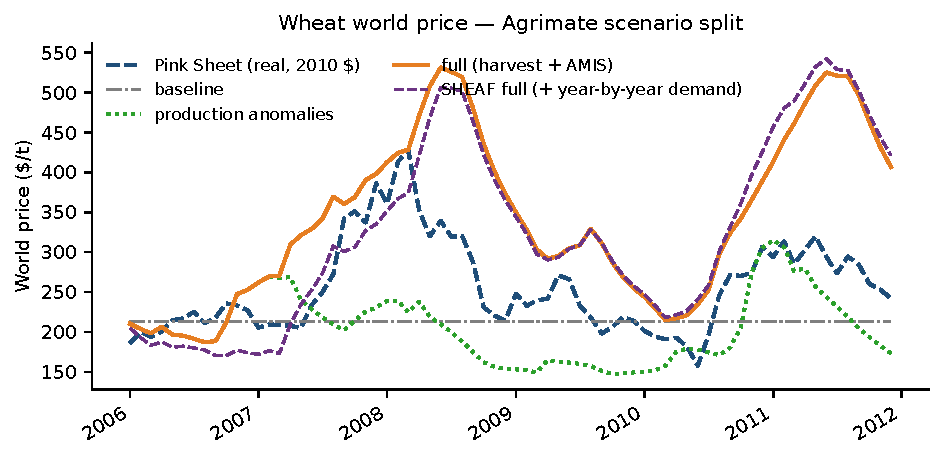
\includegraphics[width=0.98\textwidth]{fig_prices_wheat}
\caption{Wheat world price, Agrimate scenario split, versus Pink Sheet.
Grey baseline is the twin ($p_0$). Restriction, not harvest, carries 2008;
harvest carries 2010 after LOWESS detrend. Compare Kuhla et al.\ Fig.~4a
on \emph{timing and split}, not CPI dollar levels.}
\label{fig:px-wheat}
\end{figure}

\begin{figure}[H]
\centering
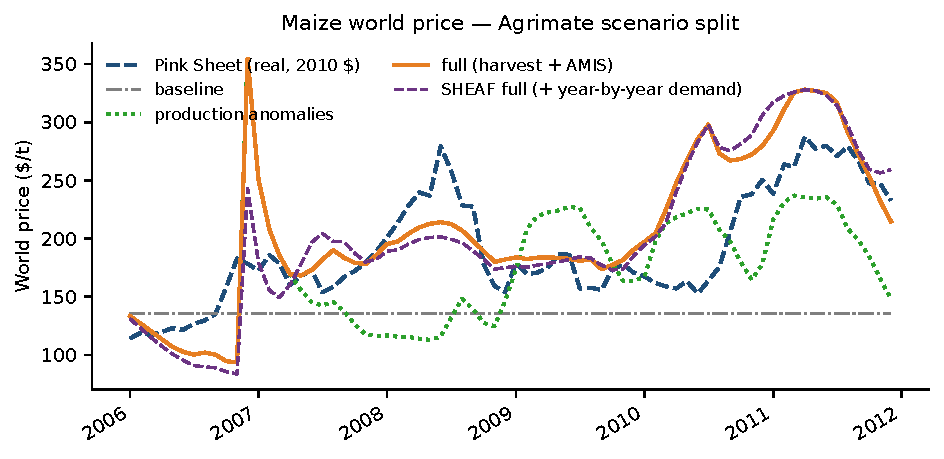
\includegraphics[width=0.98\textwidth]{fig_prices_maize}
\caption{Maize. Official full includes the USA industrial residual.
Isolated AMIS does not cut the 14-month mean price. Compare Agrimate
Suppl.\ Fig.~G.2c (their 2008 peak is restriction-led on a stable harvest;
ours is industrial-demand-led).}
\label{fig:px-maize}
\end{figure}

\begin{figure}[H]
\centering
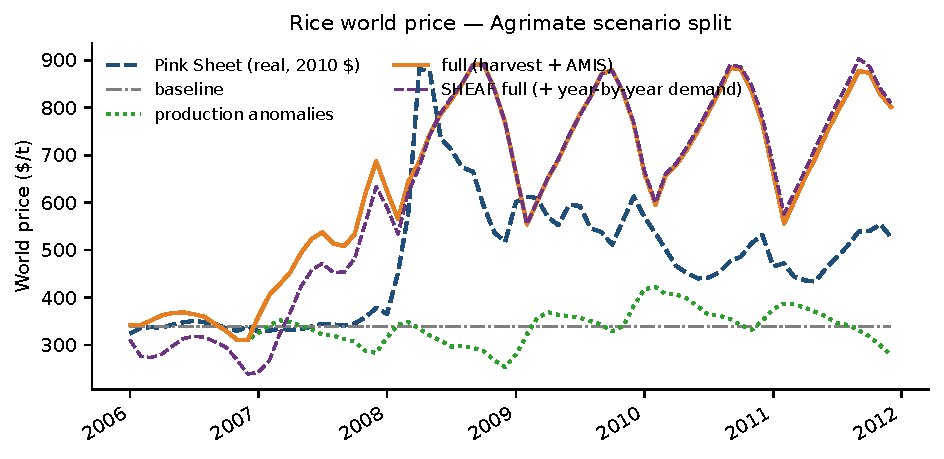
\includegraphics[width=0.98\textwidth]{fig_prices_rice}
\caption{Rice. 2008 is restriction-led on a harvest that is not a crash,
matching Agrimate Suppl.\ Fig.~G.1. 2010/11 both model and data fall.}
\label{fig:px-rice}
\end{figure}

\begin{table}[H]
\centering
\caption{Attribution: isolated legs versus official full. Isolated
\texttt{demand} is year-by-year flex+industrial with climatology harvest
and no AMIS --- a sensitivity, not the official split.}
\label{tab:attr}
\small
% Isolated legs vs official full. Isolated maize/wheat/rice \tau has industrial off.
% Hike windows: 2006-06 vs 2008-03; 2009-06 vs 2011-02 (3-month means).
\begin{tabular}{l l rrrr}
\toprule
Crop & crisis & harvest-only & AMIS-only & yoy demand & full \\
\midrule
wheat & 2007/08 & $\times 1.20$ & $\times 1.70$ & $\times 0.98$ & $\times 2.27$ \\
wheat & 2010/11 & $\times 1.85$ & $\times 1.36$ & $\times 1.35$ & $\times 1.45$ \\
maize & 2007/08 & $\times 1.11$ & $\times 1.10$ & $\times 1.46$ & $\times 1.97$ \\
maize & 2010/11 & $\times 1.01$ & $\times 0.92$ & $\times 1.12$ & $\times 1.70$ \\
rice  & 2007/08 & $\times 0.93$ & $\times 1.75$ & $\times 1.21$ & $\times 1.72$ \\
rice  & 2010/11 & $\times 1.06$ & $\times 0.81$ & $\times 1.60$ & $\times 0.82$ \\
\bottomrule
\end{tabular}

\end{table}

\paragraph{Wheat.}
2007/08 is restriction-led ($\tau\times 1.70$ versus harvest $\times 1.20$).
The full hike $\times 2.27$ overshoots observed $\times 1.82$; we do not
damp it with a 2008 dummy. 2010/11 is production-led after detrend
(harvest $\times 1.85$). The June~2009--February~2011 ratio also lifts 2009
via lingering AMIS, so restriction looks weaker on the ratio than in
levels. Agrimate's narrative treats 2007 as more production-led than we
do; we do not relabel 2008 to match them. Monthly correlation $+0.72$ is
the highest of the three crops.

\paragraph{Maize.}
2007/08 full $\times 1.97$ versus observed $\times 1.84$. Isolated harvest
and isolated AMIS are both $\sim\times 1.1$; year-by-year demand is
$\times 1.46$. The official full's extra lift is the USA industrial
block interacting with harvest and AMIS. That is a different story from
Agrimate Suppl.~G.2 (restriction-led 2008 on a stable harvest). Both can
be true of their respective models; they are not the same identification.
Isolated $\tau\times 1.10$ does not cut the 14-month mean --- the maize
assert that forbids reversing the AMIS channel. 2010/11 full $\times 1.70$
versus $\times 1.44$ is high; harvest-only is $\times 1.01$.

\paragraph{Rice.}
2008 $\times 1.72$ versus $\times 1.84$, $\tau\times 1.75$, harvest
$\times 0.93$: restriction-led, Agrimate-aligned. 2010 both series decline
($\times 0.82$ versus $\times 0.79$). Forcing year-by-year demand
\emph{worsens} 2010 (sensitivity $\times 1.60$). Headline rice therefore
keeps mean flex.

\subsection{Forcing, Russia--Egypt, regional signs}

\begin{figure}[H]
\centering
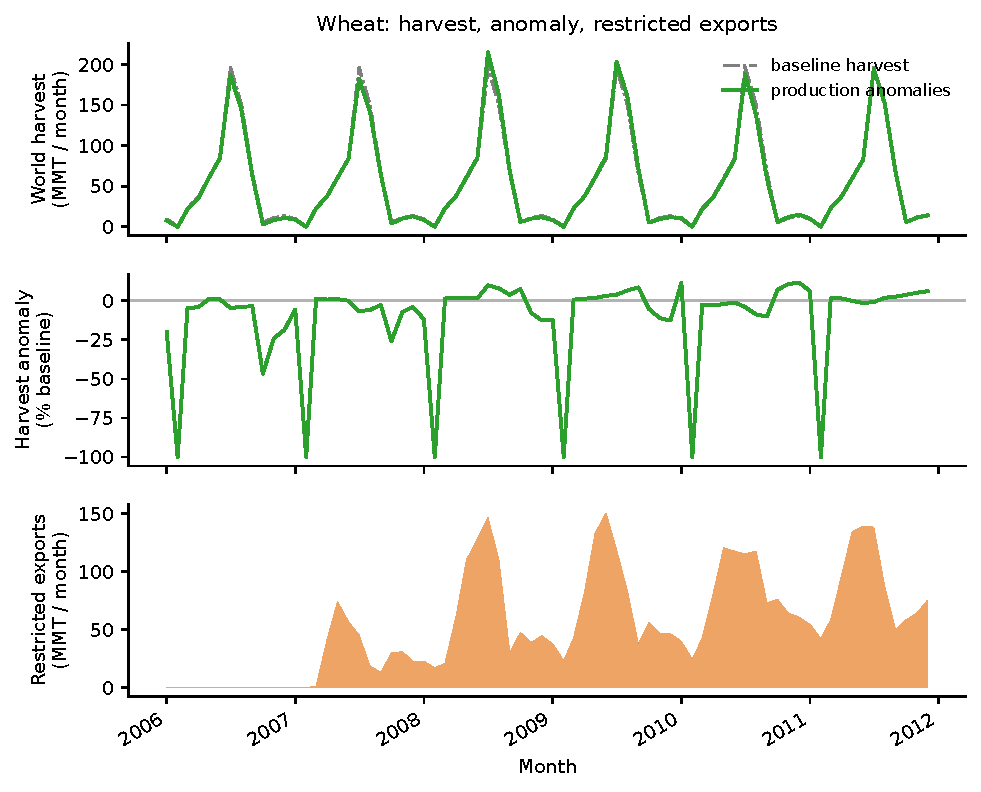
\includegraphics[width=0.98\textwidth]{fig_forcing_wheat}
\caption{Wheat harvest (climatology vs realized), LOWESS anomaly, and
AMIS-implied restricted export volume $O\tau/(1-\tau)$. Compare Kuhla et
al.\ Fig.~3.}
\label{fig:force-wheat}
\end{figure}

\begin{figure}[H]
\centering
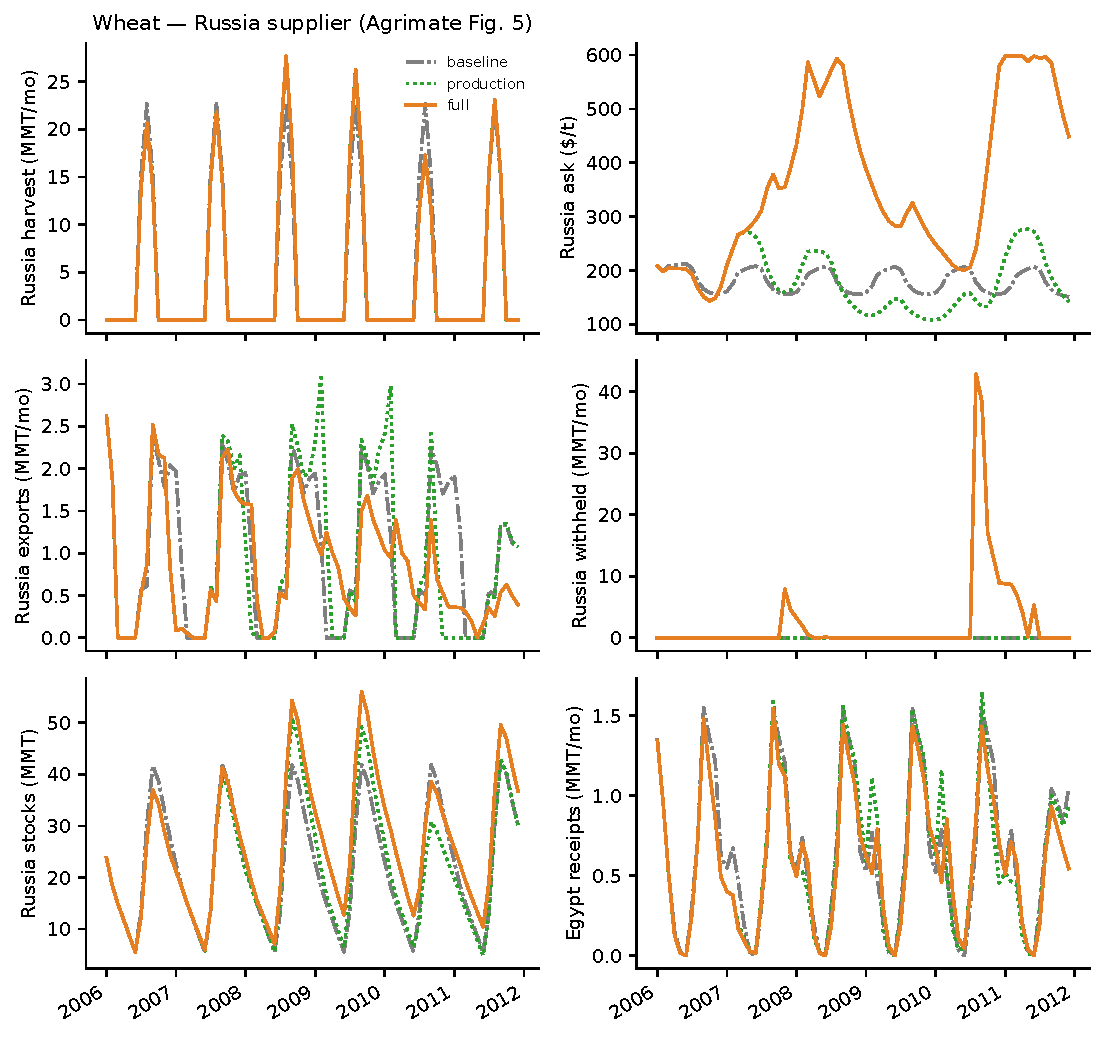
\includegraphics[width=0.98\textwidth]{fig_russia_wheat}
\caption{Russia wheat: harvest, ask, exports, withheld volume, stocks, and
Egypt receipts. SHEAF has one ask per exporter (no separate domestic vs
international offer). Compare Kuhla et al.\ Fig.~5.}
\label{fig:ru}
\end{figure}

\begin{figure}[H]
\centering
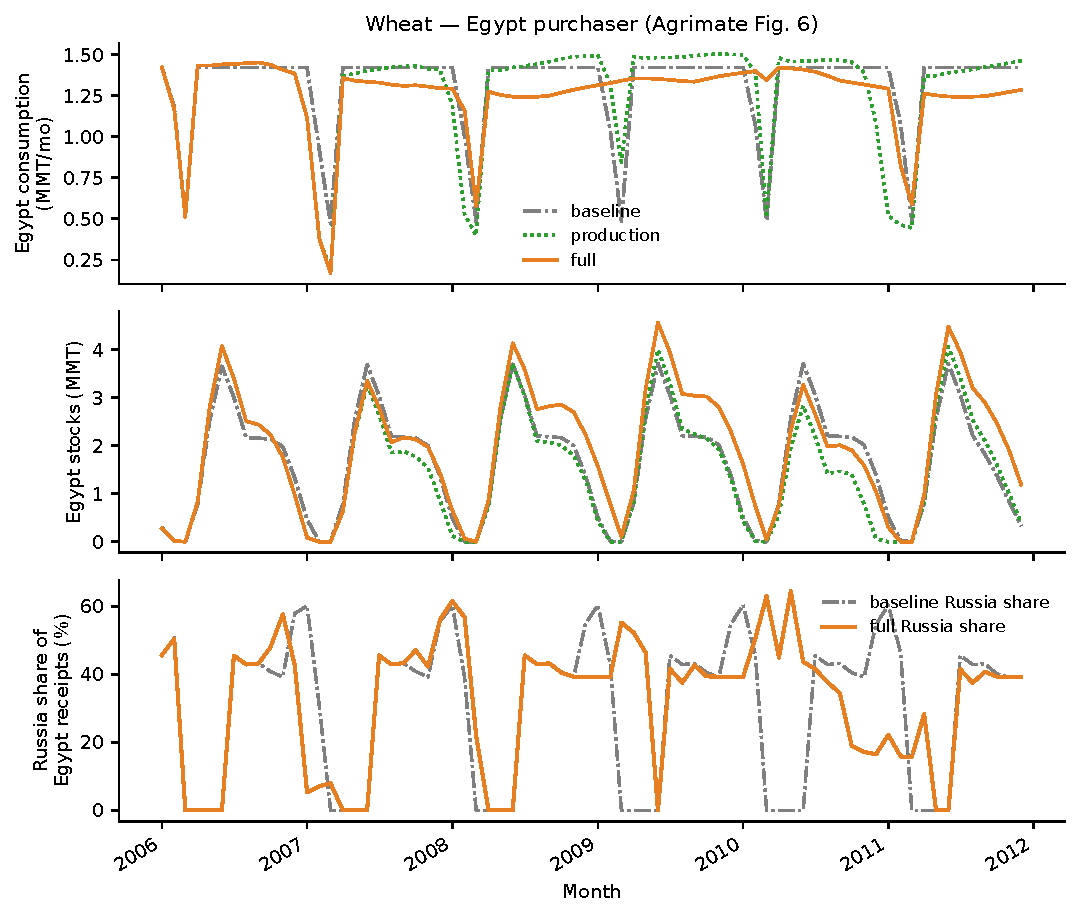
\includegraphics[width=0.98\textwidth]{fig_egypt_wheat}
\caption{Egypt wheat consumption, stocks, and Russia's share of receipts.
The 2010 ban cuts that share --- the mechanism check passes. Compare
Kuhla et al.\ Figs.~6--7.}
\label{fig:eg}
\end{figure}

Russia's share of Egypt's wheat receipts drops in 2010/11 under AMIS. That
is the Agrimate Figs.~5--7 object we can compute on 17+RoW nodes. We do
not reproduce their 28-region 2007 maps; node-level production and
stock-change signs versus PSD are the substitute (figures in the Agrimate
companion folder).

\subsection{Stocks, consumption, shipments}

\begin{table}[H]
\centering
\caption{World MY-end stocks versus PSD (crop default month), FAO/AMIS
tightness excluding China, and calendar-year consumption versus
country-sum PSD. Consumption is a P1 expansion, not Agrimate Fig.~4.}
\label{tab:stu}
\small
\begin{tabular}{l rrrr rrr}
\toprule
 & \multicolumn{4}{c}{MY-end stocks vs PSD} & \multicolumn{3}{c}{world use vs country-sum PSD} \\
\cmidrule(lr){2-5}\cmidrule(lr){6-8}
Crop & month & incl.\ China & ex-China & China share & mean ratio & corr & $\Delta$cons sign \\
\midrule
wheat & May & $\times 1.02$ & $\times 1.09$ & 28\% & $\times 0.92$ & $-0.17$ & 3/5 \\
maize & Aug & $\times 1.08$ & $\times 1.49$ & 35\% & $\times 0.92$ & $-0.64$ & 2/5 \\
rice  & Aug & $\times 1.05$ & $\times 1.14$ & 44\% & $\times 0.86$ & $-0.74$ & 1/5 \\
\bottomrule
\end{tabular}

\end{table}

\begin{figure}[H]
\centering

\includegraphics[width=0.98\textwidth]{fig_gate0_wheat_world_consumption}
\caption{Wheat world calendar-year use: official matched (mean flex +
isoelastic) versus country-sum PSD. 2006 is $\times 1.00$; the path then
falls while PSD rises. The gap is the demand system, not warehouse
rationing.}
\label{fig:cons-wheat}
\end{figure}

World MY-end stocks are on the PSD bar (wheat $\times 1.02$, maize
$\times 1.08$, rice $\times 1.05$). Ex-China wheat $\times 1.09$ and rice
$\times 1.14$ sit next to the including-China bar. Maize ex-China
$\times 1.49$ is leftover: the world snapshot is August, China maize
USDA MY-end is September, so the snapshot under-subtracts China, and
local-MY China maize is separately fat ($\sim\times 2.8$). That is not a
reason to retune the warehouse.

Consumption mean ratios $\times 0.86$--$0.92$ hide a falling model path
versus rising PSD (correlations negative). Official split is mean flex plus
$\varepsilon<0$: when price spikes, use falls, and there is no year-by-year
food/feed forcing in the headline. Median country-year ratio is a sanity
print, not the bar. $\Delta$cons signs are 3/5, 2/5, 1/5 --- not
Agrimate's ``sign corresponds except \ldots''.

\begin{table}[H]
\centering
\caption{AMIS shipment signs: official matched versus harvest-only.
Ratio $<1$ means the restriction cut that node. $\tau$ always cuts
\emph{offers}; cleared shipments are demand-constrained.}
\label{tab:ship}
\small
% Official matched (harvest+AMIS) vs harvest-only. Ratio $<1$ means AMIS cut that node.
\begin{tabular}{ll rrr}
\toprule
Crop & window & $\bar\tau$ & offer ratio & ship ratio \\
\midrule
wheat & Russia Aug--Dec 2010 & $0.95$ & $\times 0.11$ & $\times 0.79$ \\
wheat & Ukraine quota Oct 2010--Jun 2011 & $0.70$ & $\times 1.23$ & $\times 1.43$ \\
maize & Argentina May 2007 & $0.70$ & $\times 0.30$ & $\times 0.99$ \\
maize & Argentina quota May 2007--Jan 2008 & --- & $\times 0.32$ & $\times 0.89$ \\
rice  & VN+IN Oct--Dec 2007 (ban+harvest) & --- & $\times 0.06$ / $\times 0.09$ & $\times 0.26$ / $\times 0.77$ \\
rice  & Vietnam tax Sep--Nov 2008 & $0.50$ & $\times 0.57$ & $\times 0.77$ \\
rice  & India lingering Oct 2008--Sep 2011 & --- & $\times 0.31$ & $\times 1.93$ \\
\bottomrule
\end{tabular}

\end{table}

\begin{figure}[H]
\centering

\includegraphics[width=0.98\textwidth]{fig_gate0_wheat_shipments}
\caption{Wheat offer and shipment ratios, AMIS on versus harvest-only.
Russia Aug--Dec 2010 offers fall to $\times 0.11$; shipments to $\times 0.79$.
Calendar 2010 model exports remain $\times 2.39$ versus PSD (4.0~MMT).}
\label{fig:ship-wheat}
\end{figure}

The sign check that Gate~0 owns is offer-side. Russia 2010, Argentina May
2007, and Vietnam/India Oct--Dec 2007 ban+harvest all cut offers.
Shipments often move less (Armington fill is the bottleneck). Failures we
do not hide: Ukraine wheat quota \emph{raises} model shipments
($\times 1.43$); India rice lingering Oct~2008--Sep~2011 leaks
(ships $\times 1.93$); Russia calendar 2010 is still more than twice PSD.
Those are network-and-demand leftovers, not warehouse knobs.

\section{Results: Ukraine war, 2021--2023}
\label{sec:ukraine}

Agrimate's 2022 wheat exercise is Suppl.\ Fig.~A.5. We run all three
grains on locked \texttt{CropParams}, official split, stocks seeded from
2020 PSD, FAOSTAT E0 from 2019--21, and $p_0=$ 2021 Pink Sheet mean. The
hike metric is June 2021 versus May 2022 (3-month means), covering the
February invasion, Russia's March wheat/maize prohibitions, and India's
May 2022 wheat prohibition. War-related production drops enter through
LOWESS harvest anomalies in PSD; logistics disruption that is \emph{not}
an AMIS policy class is not in $\tau$. That is a limitation, not a hidden
shock.

\begin{table}[H]
\centering
\caption{2021--23 Ukraine-war window. Same \texttt{CropParams} as 2006--11.
Hike: June 2021 vs May 2022. Source:
\texttt{scripts/score\_ukraine\_war.py}.}
\label{tab:ukr}
\small
% auto-generated by scripts/score_ukraine_war.py
\begin{tabular}{l rrrrr}
\toprule
Crop & obs hike & full & harvest-only & AMIS-only & full corr \\
\midrule
wheat & $\times$1.57 & $\times$1.61 & $\times$1.09 & $\times$1.55 & +0.69 \\
maize & $\times$1.09 & $\times$1.01 & $\times$1.03 & $\times$1.04 & +0.20 \\
rice & $\times$0.91 & $\times$0.99 & $\times$0.99 & $\times$0.98 & +0.61 \\
\bottomrule
\end{tabular}

\end{table}

\begin{figure}[H]
\centering
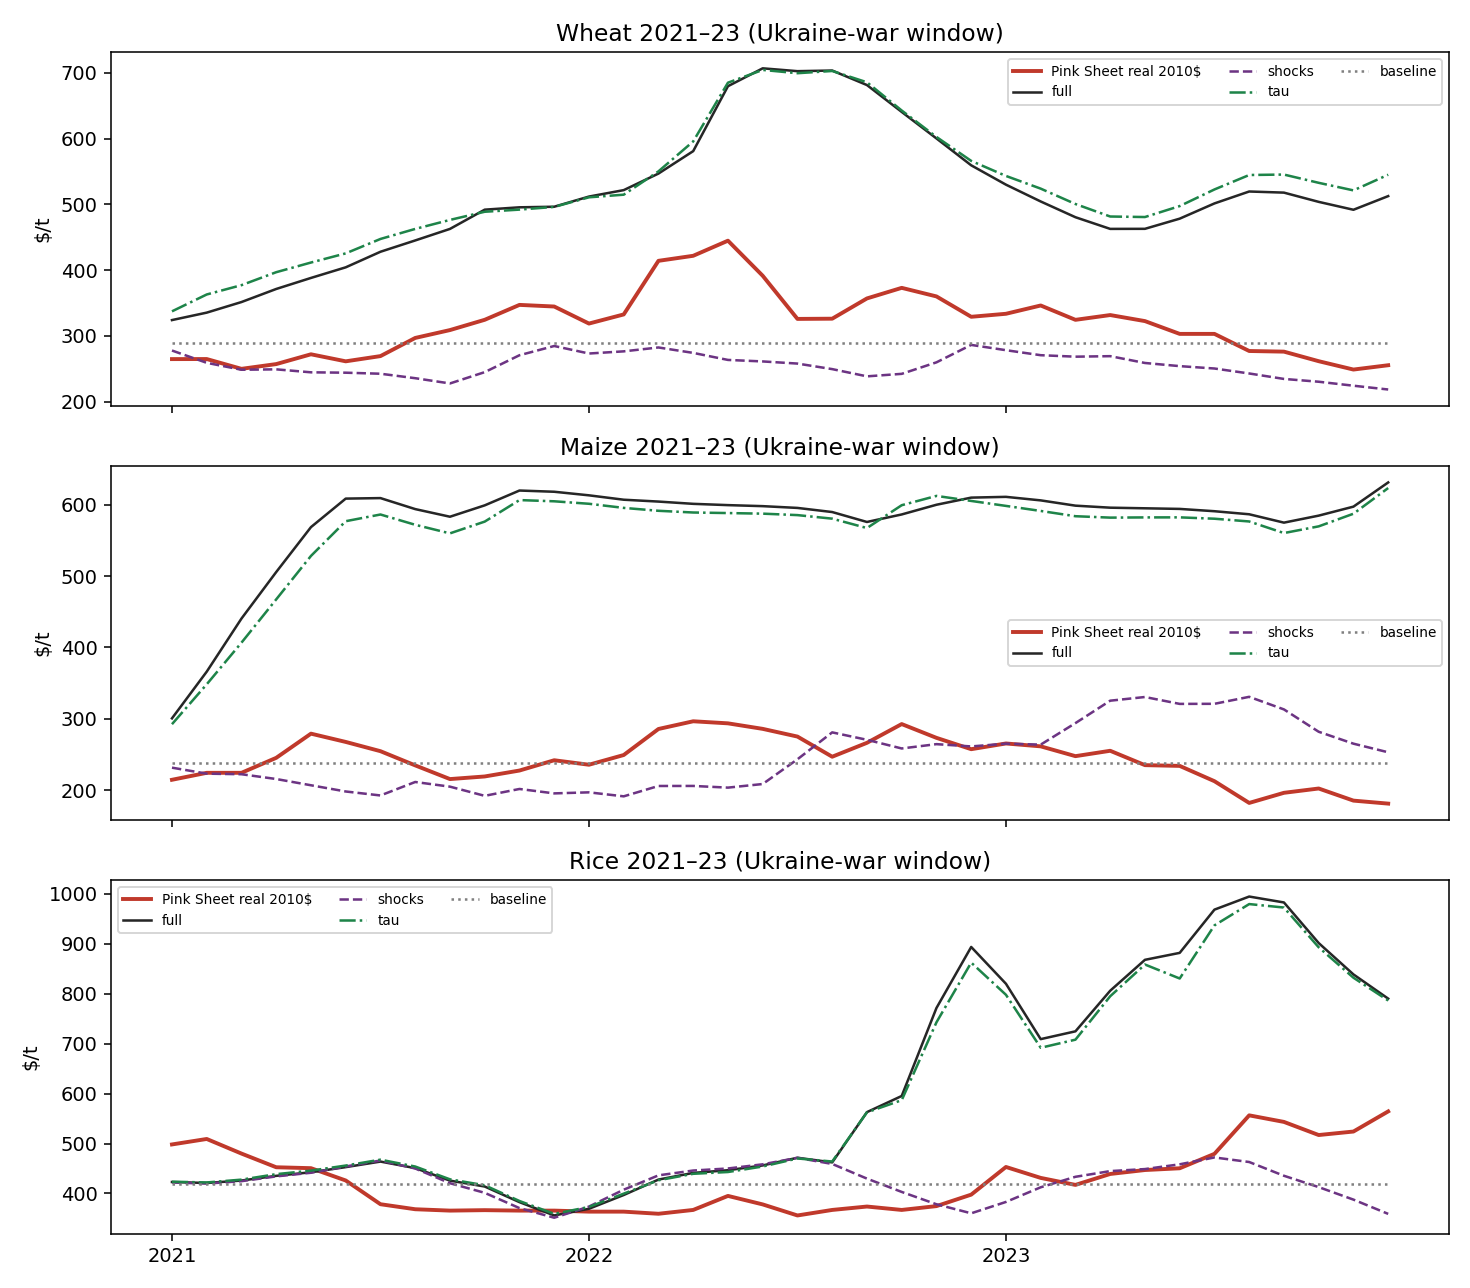
\includegraphics[width=0.98\textwidth]{fig_gate0_ukraine_prices}
\caption{2021--23 world prices, official split versus Pink Sheet.
Wheat tracks the spike and attributes it to AMIS, not harvest. Maize and
rice observed series do not spike; the model does not invent one.}
\label{fig:ukr}
\end{figure}

\paragraph{Wheat.}
Observed $\times 1.57$, full $\times 1.61$, AMIS-only $\times 1.55$,
harvest-only $\times 1.09$, correlation $+0.69$. This is a restriction-led
event on the AMIS timeline we actually have, with production anomalies
doing little in the June--May window. Parameters were not touched.

\paragraph{Maize.}
Observed hike is only $\times 1.09$. Full $\times 1.01$, correlation
$+0.20$. A weak observed move plus a 2019--21 maize network that need not
match 2022 flows is not a fail of the 2008 maize industrial story.

\paragraph{Rice.}
Observed price \emph{fell} ($\times 0.91$). Full $\times 0.99$, correlation
$+0.61$. India's later 2022 rice measures sit partly after the May 2022
hike window; we do not slide the window to catch them.

\section{Performance in the context of TWIST and Agrimate}
\label{sec:compare}

\paragraph{TWIST.}
TWIST is annual, single-commodity, no network, no AMIS~\citep{schewe2017}.
Gate~0 is not a TWIST clone and should not be scored as one. Where TWIST
is the right comparison is storage philosophy: both (and Agrimate) use
operational stock rules rather than a full rational-expectations storage
equilibrium~\citep{deaton1992}. Evaluating Gate~0 first against
Deaton--Laroque would punish a lineage choice. Evaluating it against
TWIST's annual wheat price--supply curve would ignore that we resolved
the network on purpose. The honest TWIST statement is: we inherited the
storage-as-cover idea and discarded the closed-form annual price curve
because Agrimate showed the fortnightly network is first-order for
restriction crises~\citep{headey2011,kuhla2025}.

\paragraph{Agrimate, objects we share.}
Clock, LOWESS harvest, AMIS class map, three-way scenario split, Fig.~3
withheld grain, Fig.~4a-style price panels, Russia--Egypt mechanism, and
Supplement~G rice/maize splits are the shared bar. On those objects:

\begin{itemize}
\item \textbf{Rice 2008} restriction-led on a non-crash harvest --- aligned.
\item \textbf{Wheat 2010} production-led after detrend --- aligned with
      Agrimate's 2010 reading; our 2008 wheat is more restriction-led than
      their 2007 production-led narrative.
\item \textbf{Maize 2008} is \emph{not} aligned: Agrimate restriction-led,
      SHEAF official split industrial-demand-led. Isolated SHEAF AMIS does
      not carry 2008 maize. That is a model-class difference (RFS residual
      versus their restriction channel), disclosed, not patched.
\item \textbf{Twin / baseline.} Agrimate's unperturbed run still wiggles
      with harvest and storage cost. Ours is an identity at $p_0$. Visual
      comparison of grey baselines is therefore invalid; compare treatment
      deviations.
\item \textbf{Price deflator.} MUV 2010\$ versus CPI. Compare ratios and
      correlation, not levels.
\item \textbf{Stocks.} World MY-end levels versus PSD are tight. Global
      \emph{change} signs are mixed (companion Overleaf
      \texttt{gate0\_agrimate} table: wheat stock-change 4/5 years, maize
      5/5, rice 3/5; supply-change 3/6 all crops). Agrimate's published
      language is stronger than our sign counts.
\item \textbf{28-region maps} --- we cannot replicate; 17+RoW bars only.
\item \textbf{Suppl.~F sensitivity} --- not reproduced.
\item \textbf{2022 wheat} --- we run it; hike matches. Agrimate A.5 is
      wheat-only; we add maize and rice as negative controls.
\end{itemize}

\paragraph{Agrimate, objects they did not score that we do.}
World consumption levels versus PSD; exporter shipment signs versus
harvest-only and versus PSD volumes; world stocks excluding China. Those
are P1 expansions. They make Gate~0 look \emph{worse} than a price-only
score, which is the point of expanding P1. Consumption trend and some PSD
export levels are not green (\S\ref{sec:leftovers}).

\paragraph{What ``as good as Agrimate'' would require.}
Matching their maize 2008 attribution under \emph{their} scenario split
(no ethanol residual), matching wheat 2007/08 amplitude without overshoot,
matching stock-change language, and a seasonal unperturbed baseline. We
do not currently claim that. We claim: the same checks run; rice 2008 and
wheat 2010 attribution and 2022 wheat hike are in agreement; maize 2008
identification differs for a documented structural reason; leftovers are
listed.

\section{Leftovers (structural, not a retune list)}
\label{sec:leftovers}

\begin{itemize}
\item Wheat 2007/08 still high ($\times 2.27$ versus $\times 1.82$).
\item Wheat 2006/07 residual tightness versus trend (harvest-only still
      $\times 1.46$ versus observed $\sim\times 0.95$ in that window).
\item Exporter commercial stocks on the global STU floor.
\item $\Delta$stock signs at country-year resolution near a coin-flip.
\item Consumption path versus PSD trend (mean flex + isoelastic).
\item AMIS shipment \emph{levels} versus PSD (Russia 2010 $\times 2.39$);
      India rice lingering leak; Ukraine 2010 quota ships up.
\item Maize ex-China MY-end $\times 1.49$ (month mismatch + fat China).
\item Vietnam rice stocks $\times 6$ already in \textbf{2006}, before AMIS.
      India is the AMIS lock on rice stocks.
\item Prescribed FAOSTAT E0 (P2 later).
\item No convenience yield / futures smoothing.
\item Ukraine 2022: AMIS classes only; wartime logistics outside AMIS are
      not in $\tau$. Maize/rice 2022 are weak observed moves.
\end{itemize}

None of these is a license to fit 2008. Substitution is not a patch for
them: it is a cross-crop claim that requires this spine to stay honest.

\section{Conclusion}
\label{sec:conc}

Gate~0 is complete enough to write down. With substitution off and
strategy off, a 24-step Armington spine with LOWESS harvests, an AMIS
quantity map, lean-cover storage, and ask-dominated prices hindcasts
monthly Pink Sheet correlation near $+0.7$ on 2006--11 for all three
grains, attributes 2008 wheat and rice to restrictions and 2010 wheat to
production, matches world MY-end stocks, and---without retuning---matches
the 2022 wheat hike as an AMIS event. It does not match Agrimate's maize
2008 story, does not track PSD consumption trends, and does not match
several exporter shipment \emph{volumes}. Those sentences are the result.
The next paper turns substitution on, on this spine, not instead of it.

\appendix
\section{Supplement: which equation lives in which function}
\label{sec:code}

This appendix is for readers who want to find the code. Line numbers refer
to \texttt{sheaf/dynamic\_crop.py} in the commit that ships with this note.
They will drift; function names are the stable map. Nothing in
\texttt{sheaf/core.py} (the annual market program, leftover year-Nash
prototype --- not the crisis game) is run by the hindcasts here.

\subsection{Entry points}

\begin{center}
\small
\begin{tabular}{p{0.42\textwidth}p{0.52\textwidth}}
\toprule
Claim & Code \\
\midrule
Official P1 run &
\texttt{scripts/score\_subannual\_crop.py --crop \{wheat,maize,rice\}}
calls \texttt{run\_crop\_dynamics(..., use\_demand=False)} with
\texttt{use\_industrial} defaulting on for USA maize. \\
Ukraine-war run &
\texttt{scripts/score\_ukraine\_war.py}:
\texttt{start\_year=2021}, \texttt{end\_year=2023},
\texttt{stock\_seed\_year=2020}, \texttt{trade\_window=(2019,2021)},
\texttt{p0} = 2021 Pink Sheet mean. \\
Parameter table &
\texttt{default\_crop\_params} (lines 139--178);
dataclass fields 77--136. Companion:
\texttt{diagnostics/GATE0\_PARAMETERIZATION.md}. \\
\bottomrule
\end{tabular}
\end{center}

\subsection{Equation map}

\begin{center}
\small
\begin{tabular}{llp{0.48\textwidth}}
\toprule
Eq.\ / object & Function (approx.\ lines) & Notes \\
\midrule
Clock $T_y=24$ & \texttt{sheaf/calendar24.py} & \texttt{STEPS\_PER\_YEAR} \\
Calendars & \texttt{sheaf/seasonal.py} \texttt{harvest\_path} & triangular months \\
LOWESS $a_{i,y}$ & \texttt{data\_usda.\_lowess} 82--101;
\texttt{detrend\_anomalies} 104--112;
\texttt{\_harvest\_anomaly\_scalars} 232--261 & tricube local linear;
per-country PSD, not world aggregate \\
Industrial~\eqref{eq:industrial} & \texttt{\_demand\_blocks} 369--418 &
USA maize FSI minus 2000--04 mean \\
Desired~\eqref{eq:desired} & \texttt{\_simulate\_window} 554--555 &
\texttt{(p/p0)**elast} on flex only \\
Lean~\eqref{eq:lean} & 541--563 &
\texttt{steps\_to\_harvest\_pulse}, \texttt{rolling\_ahead\_variable} \\
Offers~\eqref{eq:demand-offers} & 565--570 &
\texttt{cuts[:,t]} is $\tau$ \\
Warehouse~\eqref{eq:warehouse} & 588--597 &
\texttt{pipeline\_max\_steps>0} pads $H_t$; rice has 0 \\
AMIS map & \texttt{\_AMIS\_CUT} 43--50;
\texttt{amis\_export\_cuts} 299--330 & overlapping $\mapsto$ \texttt{max} \\
Vietnam rice E0 & \texttt{\_repair\_vietnam\_rice\_e0} 420--439 &
2019--21 mix, 12\% scale \\
$\tilde A$~\eqref{eq:ask-reweight} & \texttt{\_ask\_reweight\_dest} 462--468 & \\
Clear~\eqref{eq:armington} & \texttt{\_bilateral\_clear} 471--496 &
residual pool $\nu$ \\
Ask~\eqref{eq:ask} & 599--610 & clip $[0.45p_0,2.8p_0]$ \\
Free~\eqref{eq:free} & 612--618 & locked $= \tau\max(S-T,0)$ \\
$p^\star$~\eqref{eq:pstar} & 630--654 & calm $\Rightarrow p_0$;
else $\omega p^{\mathrm{tr}}+(1-\omega)p^{\mathrm{scar}}$ \\
Twin identity & \texttt{assert\_twin\_identity} 828--846 &
no harvest/AMIS/industrial $\Rightarrow$ flat $p_0$ \\
AMIS raises $p$ & \texttt{assert\_amis\_raises\_price} 848--881 &
maize: isolated $\tau$ must \emph{not} cut 14-month mean \\
AMIS cuts $O$ & \texttt{assert\_amis\_cuts\_exports} 902+ &
wheat: offers and shipments; maize/rice: offers only \\
No fake spring spike & \texttt{assert\_no\_spring\_spike} 883--900 &
climatology path \\
Local MY-end stocks & \texttt{sheaf/marketing\_years.py} &
not calendar December \\
\bottomrule
\end{tabular}
\end{center}

\subsection{What is deliberately not in this spine}

\begin{itemize}
\item \texttt{DemandSystem} / \texttt{subst\_scale} in \texttt{sheaf/core.py}
      --- substitution off.
\item \texttt{ExportRestrictionGame} --- not run. Gate~0 $\tau$ is AMIS.
      The crisis game, when on, is \texttt{dynamic\_policy.py} on this
      spine (Headey clock), not year-IBR in \texttt{core.py}.
\item \texttt{SpatialEquilibrium} QP (CLARABEL/SCS/OSQP) --- Gate~0 clears
      by Armington min, not a Takayama--Judge program.
\item \texttt{market\_responsive\_storage} / \texttt{strategic\_storage} in
      \texttt{core.py} --- Gate~0 uses lean targets + warehouse clip.
\item Convenience yield, futures, acreage response, WASDE ethanol gallons.
\end{itemize}

\subsection{Reproducing every number in this note}

\begin{verbatim}
python scripts/score_subannual_crop.py --crop wheat
python scripts/score_subannual_crop.py --crop maize
python scripts/score_subannual_crop.py --crop rice
python scripts/make_agrimate_comparison.py
python scripts/score_ukraine_war.py
python scripts/assemble_whitepaper.py
python scripts/score_whitepaper_maps.py
\end{verbatim}

Choropleths: \texttt{sheaf/maps.py}. Maps do not retune \texttt{CropParams}.

Zip \texttt{overleaf/gate0\_whitepaper/} and upload to Overleaf
(New Project $\to$ Upload Project). Do not upload gitignored Agrimate PDFs.


\bibliography{refs}

\end{document}
